\chapter{ทฤษฎีความรู้และงานที่เกี่ยวข้อง}

\emph{หัวข้อต่าง ๆ ในแต่ละบทเป็นเพียงตัวอย่างเท่านั้น หัวข้อที่จะใส่ในแต่ละบทขึ้นอยู่กับโปรเจคของนักศึกษาและอาจารย์ที่ปรึกษา}

ตัวอย่างการใส่อ้างอิงที่มา -> \cite{hypersense} ถ้าต้องการใส่แหล่งอ้างอิงมากกว่า 1 ให้ทำดังนี้ -> \cite{hypersense,bworld}
อธิบายทฤษฎี องค์ความรู้หลักที่ใช้ในงาน งานวิจัยที่นำมาใช้ในโครงงาน หรือเปรียบเทียบผลิตภัณฑ์ที่มีอยู่ในท้องตลาด\cite{bworld}
Explain theory, algorithms, protocols, or existing research works and tools related to your work.


% \section{ระบบแนะนำสินค้า}

% \begin{table}[!h]
%     \caption{test table method1}\label{tbl:method1}
%     \begin{tabular}{c|c|l|rr} \hline\hline
%         Center & Center & left aligned & Right & Right aligned \\ \hline\hline
%         Center & Center & left aligned & Right & Right aligned \\ \hline
%         Center & Center & left aligned & Right & Right aligned \\
%         Center & Center & left aligned & Right & Right aligned \\ \hline
%         Center & Center & left aligned & Right & Right aligned \\ \hline\hline
%     \end{tabular}
% \end{table}

\section{อัลกอริทึมในการแปลผลภาษา}
\subsection{Term Frequency Inverse Document Frequency (TF-IDF)}
เป็นอัลกอริทึมที่ผสมผสานกันระหว่าง Term-Frequency (TF) และ Inverse Document Frequency (IDF) ซึ่งเป็น
เทคนิคพื้นฐานเทคนิคหนึ่งที่ใช้ในการวิเคราะห์ค้นหาคำสำคัญของข้อมูลในลักษณะของข้อความ
\begin{itemize}
    \item \textbf{Term-Frequency (TF)} โดยจะคำนวณเป็นอัตราส่วนของจำนวนคำนั้น ๆ ต่อจำนวนคำทั้งหมดในเอกสาร
    เพื่อหาว่าคำนั้นมีความถี่เท่าไหร่
    \begin{figure}[!h]\centering
        \setlength{\fboxrule}{0.2mm} % can define this in the preamble
        \setlength{\fboxsep}{1cm}
        \fbox{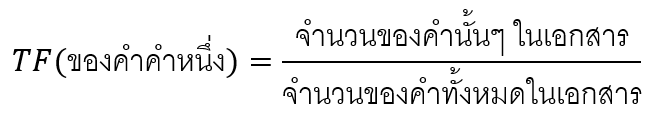
\includegraphics[width=5cm]{./figure/figure_tf.png}}
        \caption{สมการการคำนวณ Term-Frequency (TF)}\label{fig:model4}
    \end{figure}
    \item \textbf{Inverse Document Frequency (IDF)} โดยจะคำนวณความสำคัญของแต่ละคำโดยคำที่พบได้บ่อยจะมีค่า IDF ที่ต่ำ
    ซึ่งบ่งบอกว่าคำเหล่านั้นไม่สามารถดึงเอาจุดเด่นของเอกสารออกมาได้ดี
    \begin{figure}[!h]\centering
        \setlength{\fboxrule}{0.2mm} % can define this in the preamble
        \setlength{\fboxsep}{1cm}
        \fbox{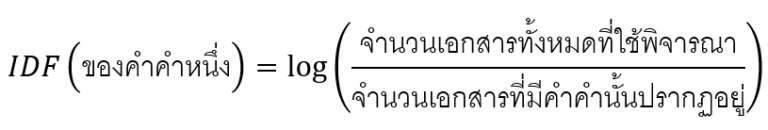
\includegraphics[width=5cm]{./figure/figure_idf.png}}
        \caption{สมการการคำนวณ Inverse Document Frequency (IDF)}\label{fig:model5}
    \end{figure}
    \item \textbf{คำนวณค่า TF-IDF} โดยเราจะนำ TF กับ IDF มาคำนวณและถ้าหากคำไหนที่มาค่า TF-IDF ที่สูง จะถูกมองว่าเป็นคำที่มีความสำคัญ
    สูง (กล่าวถึงบ่อย แต่ก็ไม่ได้ปรากฏอยู่หลายเอกสารเกินไป) และมีแนมโน้มจะเป็นใจความสำคัญของเอกสาร
    \[TFIDF = TF * IDF\]
\end{itemize}


\section{อัลกอริทึมในการแยกประเภทเรซูเม}
\subsection{อัลกอริทึม I K-Nearest Neighbors (KNN)}

% Can define this in the preamble..
เป็นอัลกอริทึมสำหรับการจัดกลุ่มข้อมูล (Classfication) ซึ่งอยู่ในกลุ่มของการเรียนรู้แบบมีผู้สอน (Supervised Learning)
หลักการทำงาน คือการจัดกลุ่มโดยอิงถึงความใกล้เคียงของข้อมูล เพื่อคาดเดาหรือจำแนกประเภทข้อมูลใหม่ โดยหลักการทำงานสามารถสรุปได้ดังนี้
\begin{enumerate}
    \item  เลือกค่า K : กำหนดค่า K ที่ต้องการ ซึ่งเป็นจำนวนของข้อมูลที่ใกล้ที่สุดที่จะใช้ในการตัดสินใจ
    \item  คำนวณระยะทาง : ใช้ระยะทางยูคลิเดียน (Euclidean distance) เพื่อคำนวณหาความคล้ายคลึงระหว่างข้อมูล
    \item  หาข้อมูลที่ใกล้ที่สุด : หลังจากคำนวณระยะทางระหว่างข้อมูลทดสอบกับข้อมูลในชุดข้อมูลการฝึกฝน เราจะเลือกข้อมูล K รายการที่มีระยะทางน้อยที่สุด
    \item  คำนวณผลโหวต : เมื่อเราได้ข้อมูล K รายการที่ใกล้ที่สุดแล้ว เราจะนับจำนวนรายการในแต่ละกลุ่มหรือประเภทข้อมูล 
    และกำหนดกลุ่มหรือประเภทข้อมูลของข้อมูลทดสอบตามจำนวนที่มากที่สุดใน K รายการนั้น
    \item  ทำนายผลลัพธ์ : สุดท้ายเราก็จะได้กลุ่มข้อมูลที่ถูกแบ่งออกมาพร้อมใช้ในการทำนายต่อไป
\end{enumerate}

\begin{figure}[!h]\centering
    \setlength{\fboxrule}{0.2mm} % can define this in the preamble
    \setlength{\fboxsep}{1cm}
    \fbox{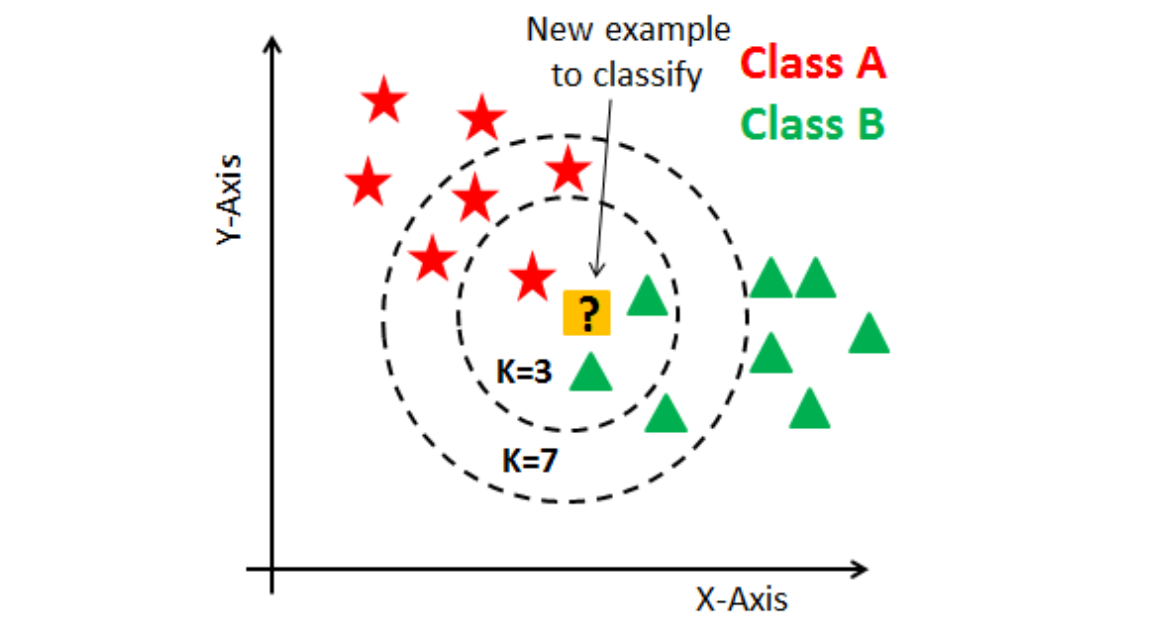
\includegraphics[width=5cm]{./figure/figure_knn.png}}
    \caption{ลักษณะการทำงานของ K-Nearest Neighbors}\label{fig:model2}
\end{figure}

\subsection{อัลกอริทึม II Naive Bayes Classifier}
Naive Bayes Classification เป็นหนึ่งใน Classification Model ใช้ในการแบ่งกลุ่มหรือหาเหตุการณ์ที่จะเกิดขึ้นโดยการอิงทฤษฎีความน่าจะเป็นของ 
Bayes หรือ Bayesian 
ซึ่งจะคำนวณว่าจะเกิดเหตุการณ์นั้นหรือไม่โดยจะเพิ่มโอกาสในการเกิดเหตุการณ์เข้าไปด้วย 
โดยมักจะใช้ในการวิเคราะห์ข้อมูลที่มีความต่อเนื่องของเหตุการณ์ (Dependent Event) เช่น 
โอกาสในการเกิดโรคในกลุ่มประชากรที่เราสนใจ ซึ่งจำเป็นจะต้องอาศัยการคำนวณผ่านสูตรดังนี้ และกำหนดให้

\begin{figure}[!h]\centering
    \setlength{\fboxrule}{0.2mm} % can define this in the preamble
    \setlength{\fboxsep}{1cm}
    \fbox{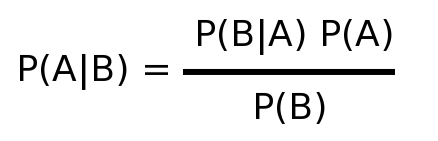
\includegraphics[width=5cm]{./figure/figure_nb.png}}
    \caption{สมการความน่าจะเป็นของ Bayes หรือ Bayesian}\label{fig:model3}
\end{figure}

P(A|B) คือความน่าจะเป็นในการเกิดเหตุการณ์ A โดยมี B เป็น Condition \\
P(B|A) คือความน่าจะเป็นในการเกิดเหตุการณ์ B โดยมี A เป็น Condition \\
P(A) คือโอกาสในการเกิดเหตุการณ์ A จากเหตุการณ์ทั้งหมด \\
P(B) คือโอกาสในการเกิดเหตุการณ์ B จากเหตุการณ์ทั้งหมด \\